%Usually an article, 12pt font, with a seperate title page
\documentclass[12pt,titlepage]{article}
%Ability to include figures easily, and eps files
\usepackage{graphicx}
\usepackage{grffile}
\usepackage{epstopdf}
\usepackage{epsfig}
\usepackage[euler]{textgreek}
%Hide links on autoref, and call each piece a section
\usepackage[hidelinks]{hyperref}
\def\subsectionautorefname{Section}
\def\subsubsectionautorefname{Section}
%Allows symbols, captions, math
% \usepackage{amssymb}
\usepackage{amsmath} %can also use to align equations
\usepackage{caption}
%Allow acronyms, with the list beneath
\usepackage[nolist,nohyperlinks]{acronym}
\begin{acronym}
\end{acronym}
%Use natbib for bibliography
\usepackage[square,super,comma,sort&compress]{natbib}
%Style changes, indent all paragraphs, use the full page size, change the section heads, nice fractions, nice tables
\usepackage{indentfirst}
\usepackage[margin=1in]{geometry}
\usepackage{setspace}
\onehalfspacing
\usepackage[small]{titlesec}
\titlelabel{\thetitle. }
\usepackage{nicefrac}
\usepackage{booktabs}
\newcommand\tab[1][1cm]{\hspace*{#1}}
%Allows for me to non-justify some regions
\usepackage{ragged2e}

% Another package for doing title of assignment --> got it from Joel
%\usepackage{titlesec}
%\titleformat{\subsection}[runin]
%{\normalfont\large\bfseries}{\thesubsection}{1em}{}
%\titleformat{\subsubsection}[runin]
%{\normalfont\normalsize\bfseries}{\thesubsubsection}{1em}{}
\usepackage{pdflscape}
\usepackage{enumitem}% http://ctan.org/pkg/enumitem
\usepackage{adjustbox}


\begin{document}

\begin{titlepage}

\newcommand{\HRule}{\rule{\linewidth}{0.5mm}} % Defines a new command for the horizontal lines, change thickness here

\center % Center everything on the page
 
%	HEADING SECTIONS

\textsc{\LARGE McMaster University}\\[1.5cm] % Name of your university/college
\textsc{\Large MECHTRON 4TB6A}\\[0.5cm] % Major heading such as course name
\textsc{\large Mechatronics \& Software Engineering Capstone}\\[0.5cm] % Minor heading such as course title

%	TITLE SECTION
\vspace{1cm}
\HRule \\[0.2cm]
{ \Large \vspace{0.25cm}  \textsc{  \LARGE System Requirements} \vspace{0.3cm} }  % Title of your document
\HRule \vspace{1cm}

\textsc{\LARGE Health Mate - Pill Dispenser}
 
 \begin{figure}[h]
  \centering
  
\includegraphics[width=.4\linewidth]{../ApexEngineering.png}
\end{figure}
 \vspace{1cm}
 
%----------------------------------------------------------------------------------------
%	AUTHOR SECTION
%----------------------------------------------------------------------------------------

\begin{table}[ht!]
\centering
\begin{tabular}{c c c}
\toprule
\textbf{Name} & \textbf{Student Number} & \textbf{McMaster Email}         \\ \midrule
Justin Ballaro & 400015482 & ballaroj@mcmaster.ca \\
Joel Bates & 001420696 & batesjj@mcmaster.ca \\
Brodie Bresette & 400029059 & bresettb@mcmaster.ca \\
Nicholas D'Angelo & 400018631 &  dangelon@mcmaster.ca  \\
Daniel Pietrangelo & 400010287 &  pietrand@mcmaster.ca \\
  \bottomrule
\end{tabular}
\label{Tab:HU}
\end{table}

%	DATE SECTION
\vfill
{\large Sunday, November 1, 2020}\\[3cm] % Date, change the \today to a set date if you want to be precise
 % Fill the rest of the page with whitespace

\end{titlepage}

\pagebreak
\pagenumbering{roman}
\tableofcontents
\pagebreak
\pagenumbering{arabic}

\section{Table of Revisions}

\begin{table}[ht!]
\begin{center}
\begin{adjustbox}{max width=\textwidth}
\small
\begin{tabular}{|p{0.1\textwidth}|p{0.1\textwidth}|p{0.2\textwidth}|p{0.4\textwidth}|}
 \hline
 \textbf{Revision } & \textbf{Date} &
 \textbf{Authors} &
 \textbf{Revision Comments}\\
 \hline \centering
 0 & \centering
 11/1/2020 & 
 Justin Ballaro \newline
Joel Bates \newline
Brodie Bresette \newline
Nicholas D'Angelo \newline
Daniel Pietrangelo &
Inital Revision \\
\hline
\end{tabular}
\end{adjustbox}
\end{center}
\caption{Table of Revisions}
\end{table}

\pagebreak

\section{Introduction}
This document is a detailed overview of the system requirements for the Health Mate - Pill Dispenser. As the project progresses, this systems requirements overview will be updated accordingly.

\section{System Overview}
\subsection{Purpose}
The medication taken by an individual is only as effective as the abidance by the patient to take the prescribed medication at the times designated. The purpose of this project is to develop an integrated hardware and software system that dispenses a person's daily medication based on a two week schedule that is decided by a health care professional. The system will also provide an online portal for the patient and their respective health professionals to gain a new in depth overview of the patient's health. This portal will allow the respective healthcare professionals to upload the patients medication schedule. It will also display the statistics stored from the device.


\subsection{Scope}
This project's scope consists of four main components. Each component plays an integral role in the overall system. A general overview of each component can be found below:
\begin{enumerate}
    \item System for dispensing a pill from a storage container (Silo)  to a designated area.
    \item Embedded control system for initiating dispensing and collecting data statistics.
    \begin{itemize}
        \item The control system shall take action based on given schedule and type of medication.
    \end{itemize}
    \item Secure portal for creating, editing and uploading schedule to device along with viewing patient statistics.
    \item Public web platform to host patient and product educational information.
    \begin{itemize}
        \item Note: Any content creation in terms of marketing for the public facing website is out of the scope of this project. 
    \end{itemize}
\end{enumerate}

\pagebreak
\subsection{Context Diagram}
 \begin{figure}[h]
  \centering
  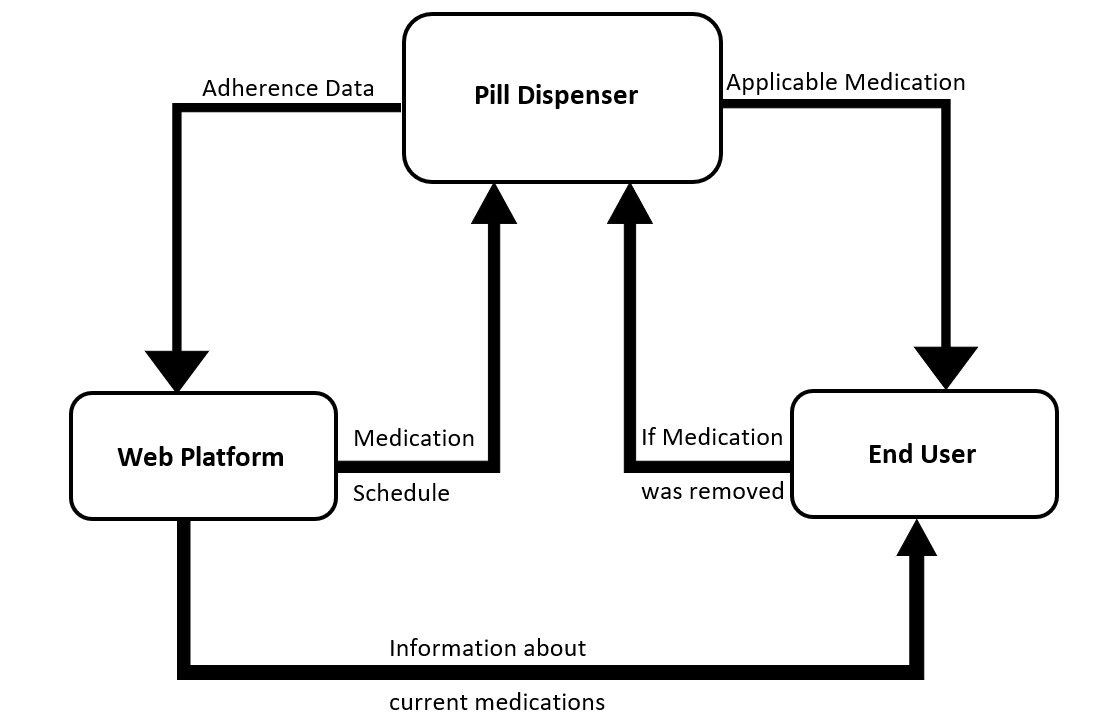
\includegraphics[width=.8\linewidth]{ContextDiagram.png}
  \caption{Context Diagram}
\end{figure}


\subsection{Monitored Variables}
\begin{table}[ht!]
\begin{center}
\begin{adjustbox}{max width=\textwidth}
\small
\begin{tabular}{|p{0.3\textwidth}|p{0.5\textwidth}|p{0.10\textwidth}|}
 \hline
 \textbf{Name} & \textbf{Description} & \textbf{Units}\\
 \hline 
Pill Collected & Sensor detecting if the pill was taken from the dispenser. & N/A\\
 \hline
 Pill Dispensed & Tracks what/how many pills are physically dispensed by the system. Determines if pills are stuck or the wrong amount has been released.  & N/A\\
 \hline
 Manual Dispense Request & Button/command used to manually dispense medication. & bool \\
 \hline
Date and Time & Needed to follow medication schedule. & dd:mm:yy hh:mm:ss\\
 \hline
Adherence & Data collected on taken/missed pills. & json string\\
 \hline
 Medication Schedule & Medication schedule based on pharmacist input. & json string\\
 \hline
User Inputs & All potential user inputs (i.e. settings menu, additional buttons). Further detail  in future revisions. & N/A\\
 \hline

\end{tabular}
\end{adjustbox}
\end{center}
\caption{Monitored variables.}
\end{table}

\subsection{Controlled Variables}
\begin{table}[ht!]
\begin{center}
\begin{adjustbox}{max width=\textwidth}
\small
\begin{tabular}{|p{0.3\textwidth}|p{0.5\textwidth}|p{0.10\textwidth}|}
 \hline
 \textbf{Name} & \textbf{Description} & \textbf{Units}\\
 \hline 
Dispensing Schedule & On-board schedule of when pills will be dispensed. & json string \\
 \hline
Prescription Silo \# & Input by the pharmacist when filling the device. Silo number will be set for each prescription. & int \\
 \hline
 Audible/Visual Alarm & Cue for user to take medication. & bool \\
 \hline
 Dispensing Mechanism & Dispenses medication from appropriate silo when scheduled. & bool\\
 \hline
\end{tabular}
\end{adjustbox}
\end{center}
\caption{Controlled variables}
\end{table}

\subsection{Constants}
\begin{table}[ht!]
\begin{center}
\begin{adjustbox}{max width=\textwidth}
\small
\begin{tabular}{|p{0.3\textwidth}|p{0.5\textwidth}|p{0.10\textwidth}|}
 \hline
 \textbf{Name} & \textbf{Description} & \textbf{Units}\\
 \hline 
 Silo Height and Width & The dimensions of each individual silo & cm\\
 \hline
 Pill Dispenser Height and Width & The overall size of the Pill Dispensing machine & cm\\
 \hline
\end{tabular}
\end{adjustbox}
\end{center}
\caption{Constant variables.}
\end{table}


\section{System Behaviour and Requirements}
\subsection{Behaviour Overview}
\vspace{-.5cm}
\begin{align*}
    PillDispenser &= f(Date/Time, DispensingSchedule, ManualRequests, Pill Collected, \\ & \ \ \ \ \ \ Pill Dispensed, UserInputs) \\ \\
    WebPlatform &= f(MedicationSchedule, AdherenceStatistics, LoginInformation, Design) %needs some work
\end{align*}
Note: A function table for the web platform will be provided once the project is farther along in progress. 

\begin{table}[ht!]
\begin{center}
\begin{adjustbox}{max width=\textwidth}
\small
\begin{tabular}{| c | c | c | c |}
\hline
  & \multicolumn{3}{c|}{\textit{Results}}\\
 \hline 
  & \textbf{Dispense} & \textbf{} & \textbf{Notify}\\
 \textit{Conditions} & \textbf{Medication} & \textbf{Record data} & \textbf{User}\\
 \hline 
 Date/Time = DispensingSchedule & TRUE & TRUE & TRUE\\
 \hline
  Date/Time != DispensingSchedule & FALSE & FALSE & FALSE\\
 \hline
  ManualRequest & TRUE & TRUE & FALSE\\
 \hline
  !ManualRequest & FALSE & FALSE & FALSE\\
  \hline
   PillCollected & FALSE & TRUE & FALSE\\
 \hline
  !PillCollected & FALSE & TRUE & TRUE\\
 \hline
 PillDispensed & FALSE & TRUE & FALSE\\
 \hline
 !PillDispensed & FALSE & TRUE & TRUE\\
 \hline
  UserInputs & X & X & X\\
 \hline
\end{tabular}
\end{adjustbox}
\end{center}
\caption{Pill Dispenser Behaviour Table}
\end{table}

\pagebreak
\subsection{Functional Decomposition}
\begin{figure}[!htbp]
    \centering
    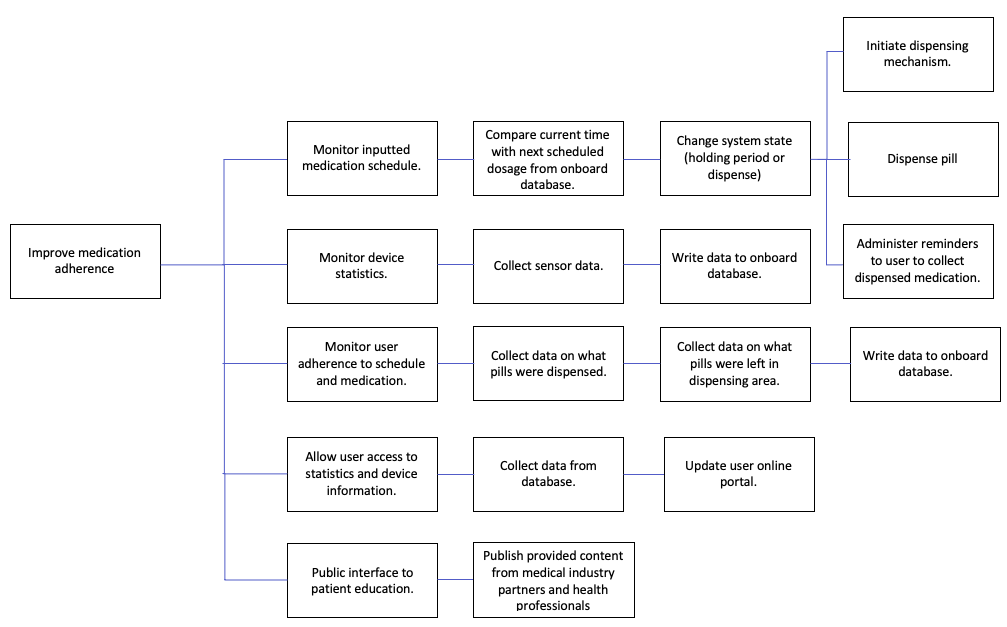
\includegraphics[width=\textwidth,height=\textheight,keepaspectratio]{FuncDecomp.png}
    \caption{Functional Decomposition Diagram}
    \label{fig:my_label}
\end{figure}


\pagebreak
\subsection{Required Behaviour Description}

\begin{table}[ht!]
\begin{center}
\begin{adjustbox}{max width=\textwidth}
\small
\begin{tabular}{|p{0.5\textwidth}|p{0.5\textwidth}|}
 \hline
 \textbf{Required Behaviour} & \textbf{Rationale} \\
 \hline 
 The system should dispense the correct number of pills when required. & 
  If not enough pills are dispensed, the client will not adhere to the given schedule. If too many pills are dispensed, the client can face serious health complications. \\
 \hline
 The system should dispense the correct pills at the correct time or time period based on a given schedule.
 \begin{itemize}
     \item The system shall store the given schedule locally after it is uploaded to the device.
 \end{itemize} &

 Dispensing the incorrect pill at a time not defined by the schedule can cause confusion for the user and potential health complications.\\
 \hline
 The system should know what pill is being dispensed. &
 The system should store this detail for use in adherence statistics. This should also allow the system to keep track of dispensing statistics.\\
 \hline
 The system must collect and store data on pill schedule adherence. & 
 Having these statistics available for the end user and their health professional will give new insight to the clients health.\\
 \hline
 The system should be safe and easy to operate for all users. &
 The device should not become an extra nuisance or unsafe for the health professional or end user. \\
 \hline
 The system must not damage any pills in the dispensing process. &
 If a pill is damaged in any step of the dispensing process, it becomes unusable and the patients medication schedule is put in jeopardy.\\
 \hline
 The user must be able to interact with the system through a web interface. &
 All system data and statistics will be displayed through this interface. This will also be the median used to upload the patients pill schedule. \\
 \hline
 
\end{tabular}
\end{adjustbox}
\end{center}
\caption{Behaviour Description Table}
\end{table}

\subsection{Performance Requirements}
\subsubsection{Pill Dispensing Control}
\begin{itemize}
    \item The dispenser will release the scheduled tablets at the scheduled time. 
    \item The dispenser will keep track of how many tablets of each medicine remain in the dispenser.
    \item The dispenser will only allow the user to take the tablet if safe to do so.
    \item Verify that a tablet was dispensed when it was scheduled to.
\end{itemize}
\subsubsection{Clock Requirement}
\begin{itemize}
    \item Keep an accurate clock to ensure the tablets are dispensed as scheduled.
    \item Be able to keep accurate clock through power outage.
\end{itemize}
\subsubsection{Software Requirement}
\begin{itemize}
    \item Securely transfer information to and from the pill dispenser and the web client.
    \item Schedule designed so it may be sent to the dispenser in easy fashion.
    \item Provide educational information for the client in an easy to access manner.
\end{itemize}

\subsection{Normal Operation}
Please note: The normal operation captured below would be encountered \textbf{after} a refill of the pill silos has been done. The refill procedure is not encapsulated. It also assumes the setup of the internal clock of the device has been done and a medication schedule has been uploaded to the system.

\begin{itemize}[leftmargin=*]
    \item The system is powered ON.
\end{itemize}
\begin{itemize}[label={}]
\item The system is plugged into power and the device is turned on. 
\end{itemize}
\begin{itemize}[leftmargin=*]
    \item Self system diagnosis and system preparation.
\end{itemize}
\begin{itemize}[label={}]
\item The system will begin a system diagnosis to ensure there are no issues present with the dispensing mechanism. This check will also ensure the micro-controller is working properly. At this step, the device will also take inventory of all pill containers present and analyze the users pill schedule to prepare for either the waiting period or dispensing time.
\end{itemize}
\begin{itemize}[leftmargin=*]
    \item Schedule dispensing time has not been reached (holding period).
\end{itemize}
\begin{itemize}[label={}]
\item In this state, the system is in a holding period. It polls the onboard RTC and compares the fetched time to the scheduled dispensing times at a set interval to determine when dispensing should occur.  
\end{itemize}
\begin{itemize}[leftmargin=*]
    \item Schedule dispensing time has been reached (dispense).
\end{itemize}
\begin{itemize}[label={}]
\item At this point, the device begins the dispensing process. The device reads what pills should be dispensed from the stored schedule and dispenses those pills using the onboard dispensing mechanism. After all dispensing is complete, the device returns to the holding state.
\end{itemize}

\subsection{Undesired Event Handling}
The safety of the pill dispensing machine is of critical importance. As such, the device must be able to account for any number of undesired events and have thoughtful, user-friendly remediation. Below is a list of undesired events that may occur and their potential remediation. The included events have been deemed as the most likely to occur.
\subsubsection{Pill Dispenser Jam}
The system should be able to determine if it has jammed, attempt to fix itself, and if unsuccessful, inform the user how to return the device to a functioning state.
\subsubsection{Power Outage}
The system should be able to account for a power outage, returning to its previous state, and resuming operation once re-powered.
\subsubsection{Release of Too Many Pills}
The system should be able to detect it has released too many of a certain pill, inform the user an error has occurred and advise next-steps for that specific pill.
\subsubsection{Data Transfer Error}
The system should be able to determine whether a data transfer error occurred when being programmed by the pharmacist, inform the programmer of the error and prompt the pharmacist to retry the data download.
\subsubsection{Pill Not Taken}
The system should be able to detect whether a pill was not taken by the user and determine whether the user should take the dosage or remove and replace it with the next dosage.

\section{Requirements Likely to Change}
\begin{itemize}
    \item The number of silos per device.
    \item The number of silo sets per device
    \item Ability to manually release pills earlier than scheduled.
    \item Access to silos by the end-user.
    \item The variety of pill sizes available to be dispensed.
    \item The inclusion of pill instructions.
    \item End-user's ability to change the on-device clock.
    \item How the device will be setup.
    \item The manner in which the schedule is updated to the device.
    \item Who has authority to setup and prepare the device for home-use.
    \item The level of detail included in preparing the pill dispensing schedule.
    \item Notifications to loved ones or care-taker.
    \item The upper-limit time required to successfully dispense a pill.
\end{itemize}

\section{Requirements Unlikely to Change}
\begin{itemize}
    \item 99.9\% effectiveness
    \item Ability to dispense the correct number of pills when required.
    \item Ability to use a schedule for the release of pills.
    \item Ability to know what type of pill is being dispensed.
    \item Ability to collect data on pill adherence.
    \item Ability to transfer data between the device and scheduling portal securely.
    \item Easy to use software for medical professionals.
    \item Easy to use dispensing machine for end-user.
    \item Ability to dispense all types of pill sizes.
    \item Notification for when to take scheduled pills.
    \item Accurate on-board clock.
    \item Cannot damage any pill type when dispensing.
    \item Fit on a counter-top.
    \item Low power consumption.
    \item Follows all mechanical and electrical safety laws.
\end{itemize}
\section{References}
No reference material was used in the creation of this document.

\end{document}